\section{Evaluierung}
\label{eval}
Die Feststellung des Erfolgs der Implementierung erfolgt in zwei Schritten. Zunächst wird in Bezug auf die bei der Konzeptionierung erarbeiteten Features betrachtet, ob alle gewünschten Funktionalitäten implementiert wurden. Daraufhin ist anhand bestimmter Kriterien zu überprüfen, ob die implementierten Features funktionieren.

\subsection{Evaluierung der umgesetzten Features}
In Kapitel \ref{konz:all_features} ist eine vollständige Liste aller gewünschter Features erfasst worden. Diese umfasst vor allem Features, die für Nutzende von Interesse sind, erwähnt aber auch Aspekte der Erweiterbarkeit und Vorbereitung auf zukünftige Entwicklung. Im folgenden wird untersucht, ob all diese Ziele erreicht werden konnten.

Das erste erwähnte Feature ist die interaktive und informative Auswahl von Bibliotheken und Werkzeugen. Wie in Abbildung \ref{fig:gwa_fragebogen} zu sehen ist, konnte ein Fragebogen umgesetzt werden, der genau diese Auswahl ermöglicht. Vorher und nachher sind weitere Fragen möglich, wobei bereits über \gls{CLI}-Argumente beantwortete Fragen nicht erneut gestellt werden, sodass die Konfiguration standardmäßig komplett interaktiv ist, aber auf Wunsch auch ohne jegliche Interaktion stattfinden kann.

Aufgrund der Typdefinition von Erweiterungen ist es unmöglich, eine Erweiterung zu \gls{GWA} hinzuzufügen, die nicht über grundlegende Metadaten verfügt, worunter insbesondere der Name der Erweiterung, ihre Beschreibung sowie ein Link zu weiteren Informationen zählen. Somit sind die Ziele der Interaktivität und der Informativität als erfüllt zu betrachten.

\begin{figure}
	\centering
		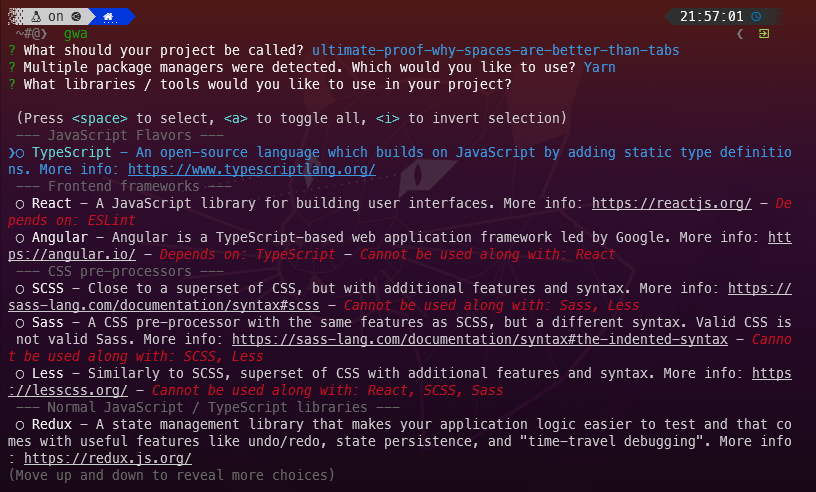
\includegraphics[width=\linewidth]{gwa-dialog.png}
	\caption{Bildschirmfoto von \gls{GWA}, nachdem der Projektname und Paketmanager festgelegt wurden. In der Aktuellen Frage ist eine Auswahl der gewünschten Bibliotheken / Werkzeuge zu treffen.}
		\label{fig:gwa_fragebogen}
  \end{figure}

Bei der Umsetzung der Fragen war außerdem darauf zu achten, dass keine unzulässige Konfiguration auswählbar ist. Dieses Feature konnte umgesetzt werden, indem nach jeder Frage die gegebene Antwort überprüft und ggf. zurückgewiesen wird. Nutzende haben im Fall einer unzulässigen Antwort dann weiterhin die Möglichkeit, ihre Antwort zu bearbeiten.

Es wäre schöner gewesen, Nutzenden bereits während der Beantwortung jeder Frage Rückmeldung zu der Gültigkeit der aktuell geleisteten Antwort zu geben. Da die für den Dialog verwendete Bibliothek jedoch kein solches Feature anbietet, wird stattdessen bei jeder Frage und ggf. neben jeder Antwortmöglichkeit angegeben, welche Einschränkungen gelten. Nutzende können basierend auf diesen Informationen versuchen, unzulässige Antworten zu vermeiden, werden aber zusätzlich beim Versuch der Einreichung jeder Antwort daran gehindert, fehlerhafte Antworten zu geben.

Diese Validierung findet auch statt, falls bestimmte Antworten schon im Rahmen der \gls{CLI}-Argumente gegeben werden. Dabei fehlschlagende Validierungen führen jedoch zu einem fehlerhaften Beenden von \gls{GWA}, um eine automatische Benutzung zu ermöglichen. Diese Entscheidung hat sich bereits bei der Erstellung automatischer Tests als hilfreich erwiesen. Auch das gewünschte Feature der Antwortvalidierung wurde also erfüllt.

Ebenfalls umgesetzt werden konnten die Auswählbarkeit des Paketmanagers sowie die Installation über Framework-spezifische \gls{CLI}s wo sie möglich ist. Damit kann, wie bereits bei der Konzeptionierung erläutert, die zukünftige Pflegbarkeit der erzeugten Projekte erleichtert werden, da die für das jeweilige Framework empfohlenen Werkzeuge genutzt werden können.

Die Umsetzung von Erweiterungen konnte nur etwas eingeschränkter geschehen. Zwar wurden mehrere verschiedene Kategorien von Erweiterungen umgesetzt, darunter Werkzeuge wie Frameworks und CSS-Präprozessoren, aber auch Bibliotheken wie RxJS. Allerdings ist ist darauf verzichtet worden, Erweiterungen für Werkzeuge und Bibliotheken zum automatischen Testen zu schreiben.

Diese Erweiterungen hätten sich von den implementierten Erweiterungen deutlich unterschieden, da sie einen großen Einfluss auf andere Erweiterungen gehabt hätten. Bei ihrer Installation hätten nämlich nicht nur die entsprechenden Werkzeuge / Bibliotheken installiert und eingebunden werden müssen, sondern es hätten sämtliche bisher existierenden Tests auf die ausgewählte Erweiterung angepasst werden müssen. Darüber hinaus hätten auch, sofern sinnvoll, von allen anderen Erweiterungen Tests basierend auf den ausgewählten Werkzeugen und Bibliotheken erzeugt werden müssen. Beispielsweise müsste demnach die Redux-Erweiterung für die erzeugten Komponenten ebenfalls Tests generieren.

Aufgrund der hohen Komplexität dieses Features und dem begrenzten, im Rahmen dieser Arbeit leistbaren Arbeitsumfangs wurde vorerst darauf verzichtet, Erweiterungen für automatische Tests umzusetzen. Diese Erweiterungen sind jedoch für die weitere Entwicklung von \gls{GWA} geplant und werden daher im Kapitel \ref{further_research} erneut thematisiert werden.

\subsection{Sicherstellung der Funktionalität}
Die Überprüfung der Korrektheit einiger Features, insbesondere der Installation von Erweiterungen, ist nur mit hohem Aufwand ausführlich möglich. Für jede Erweiterung müsste betrachtet werden, welche Installationsschritte sie durchführen soll. Häufige Schritte wie die Installation eines \gls{npm}-Pakets sind leicht zu überprüfen, aber bei außergewöhnlicheren Schritten wie der Ergänzung einer Komponente im Falle der Redux-Erweiterung müsste die erzeugte Applikation lokal gestartet werden und es müsste von Hand verifiziert werden, dass die Komponente eingefügt worden ist und über ihre erwartete Funktionalität verfügt.

Außerdem werden einige Features durch die Auswahl bzw. die Nicht-Auswahl anderer Erweiterungen aktiviert bzw. deaktiviert. Es müssen zur vollständigen Überprüfung solcher Erweiterungen also mehrere Projekte eingerichtet und überprüft werden.

Aufgrund dieses hohen Umfangs wären manuelle Tests mit einem großen zeitlichen Aufwand verbunden. Außerdem wäre die Durchführung der Tests an vielen Stellen gleich und daher anfällig für Flüchtigkeitsfehler.

Gleichzeitig ist die Automatisierung dieser Tests aufgrund ihrer Vielfältigkeit nur schwer möglich. Für viele Erweiterungen müssten spezielle Tests angefertigt werden und die Überprüfung bestimmter Features (wie die Funktionalität der durch die Redux-Erweiterung eingebundene Komponente) ließe sich am besten über Ende-zu-Ende-Tests mithilfe entsprechender Werkzeuge realisieren. Genau solche Tests sollen künftig über Erweiterungen installierbar sein, aber dann müsste man diese Tests zu diesen Evaluierungszwecken auch dann in Projekte einbauen können, wenn sie eigentlich gar nicht Teil der zu testenden Konfiguration sein sollen.

Während der manuellen Tests, die im Rahmen der Entwicklung durchgeführt wurden, hat sich jedoch gezeigt, dass sich die meisten solcher detaillierter Fehler gut durch Unit-Tests abdecken ließen. Die danach übrig gebliebenen Fehler waren ausnahmslos derart schwerwiegend, dass entweder der Installationsprozess oder das Bauen der resultierenden Applikation fehlgeschlagen hat.

Auf diese Beobachtung hin wurde eine vereinfachte Prüfung von Installationen erarbeitet, die sich leicht automatisieren lässt. Eine zu prüfende Konfiguration wird an \gls{GWA} weiter gegeben. Im Anschluss an eine erfolgreiche Installation wird das Projekt gebaut und sofern diese beiden Prozesse fehlerfrei laufen gilt das Projekt als erfolgreich eingerichtet.

Mithilfe von Docker können beliebige Konfigurationen innerhalb einer \gls{VM} durchgeführt werden. Ein TypeScript-Skript orchestriert die Erzeugung und Löschung der \gls{VM}s sowie die Ausführung der Installations- und Baubefehle innerhalb der \gls{VM}s. Im Anschluss an die automatisch durchgeführten Befehle wird jede \gls{VM} gespeichert, damit die getroffene Installation für weitere manuelle Tests zur Verfügung steht.

In diesem Skript kann festgelegt werden, welche Konfigurationen zu überprüfen sind. Da während der Entwicklung viele Probleme durch die Kombination bestimmter Erweiterungen entstanden sind, werden bei diesen Tests alle Erweiterungen in möglichst umfangreichen Projekten getestet. Unter Beachtung von Abhängigkeiten und Exklusivitäten werden also maximal viele Erweiterungen zusammen installiert.

Zum Zeitpunkt des Schreibens dieser Arbeit liegen vor allem\footnote{Außerdem ist Less nicht zusammen mit React verwendbar. Diese Kombination wird im späteren Verlauf einfach ausgelassen.} zwei Arten von Exklusivitäten vor: die zwischen Frontend-Frameworks und die zwischen CSS-Präprozessoren. Um trotz dieser Exklusivitäten alle möglichen Konstellationen überprüfen zu können, wird jede (zulässige) Kombination eines Frameworks und eines CSS-Präprozessors überprüft.

Eine weitere große Fehlerquelle war die Installation von Erweiterungen mit oder ohne TypeScript, da abhängig von TypeScript weitere \gls{npm}-Pakete zu installieren waren, besonderer Code generiert werden musste oder ähnliches. Eine Ausnahme bilden hierbei jedoch die CSS-Präprozessoren. Daher wird mit ihrer Ausnahme jede Erweiterung sowohl mit, als auch ohne TypeScript überprüft.

Aus diesen Gründen werden insgesamt acht Konstellationen von Erweiterungen überprüft: Angular wird in Kombination mit jedem der vier CSS-Präprozessoren (hier wird die Abwesenheit eines CSS-Präprozessors auch als Präprozessor gezählt) und allen sonstigen Erweiterungen installiert. Da Angular von TypeScript abhängt, werden diese Konfigurationen nie ohne TypeScript überprüft. Außerdem wird React mit jedem CSS-Präprozessor außer Less und allen übrigen Erweiterungen überprüft. Dazu kommt lediglich eine Konfiguration ohne TypeScript, da die Anwesenheit von TypeScript keinen Einfluss auf CSS-Präprozessoren hat.

Durch das Durchführen dieser Tests sind mehrere Fehler aufgefallen, die vor allem in der Kombination von CSS-Präprozessoren mit React aufgetreten sind und die vollständig behoben werden konnten. Bei der weiteren manuelle Überprüfung der dabei erstellten Projekte sind keine weiteren Fehler aufgefallen. Abschließend sind also keine Fehler bei bisher implementierten Features bekannt.